\begin{figure}[!t]
\centering
\resizebox{\columnwidth}{!}{%
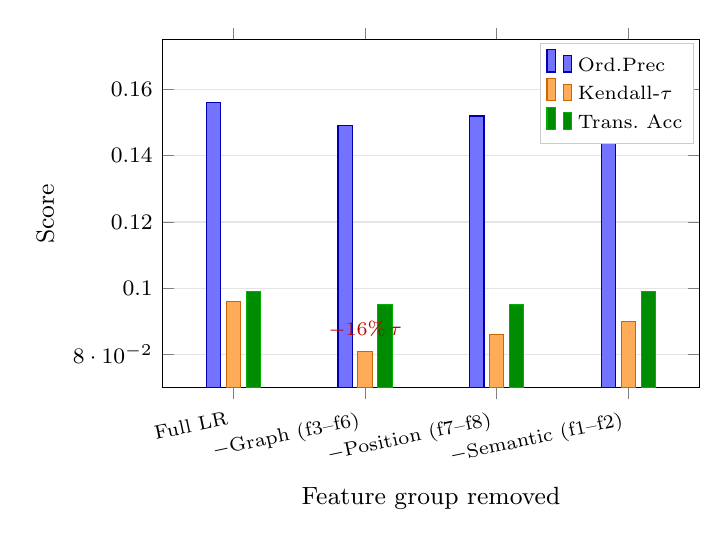
\begin{tikzpicture}
\begin{axis}[
  ybar,
  bar width=5.2pt,
  width=8.4cm, height=6.0cm,
  xlabel={Feature group removed},
  ylabel={Score},
  xlabel style={font=\small},
  ylabel style={font=\small},
  tick label style={font=\footnotesize},
  symbolic x coords={Full LR, No Graph, No Position, No Semantic},
  xtick=data,
  xticklabels={Full LR, $-$Graph (f3--f6), $-$Position (f7--f8), $-$Semantic (f1--f2)},
  xticklabel style={font=\scriptsize, rotate=12, anchor=north east},
  ymin=0.070, ymax=0.175,
  ytick={0.08,0.10,0.12,0.14,0.16},
  yticklabel style={font=\footnotesize},
  legend style={font=\scriptsize, at={(0.99,0.99)}, anchor=north east,
    inner sep=2pt, row sep=-1pt, draw=gray!40},
  legend cell align=left,
  ymajorgrids=true,
  grid style={gray!20, line width=0.4pt},
  enlarge x limits=0.18,
]

\addplot[fill=blue!55, draw=blue!70!black]
  coordinates {
    (Full LR,     0.156)
    (No Graph,    0.149)
    (No Position, 0.152)
    (No Semantic, 0.154)
  };
\addlegendentry{Ord.Prec}

\addplot[fill=orange!65, draw=orange!80!black]
  coordinates {
    (Full LR,     0.096)
    (No Graph,    0.081)
    (No Position, 0.086)
    (No Semantic, 0.090)
  };
\addlegendentry{Kendall-$\tau$}

\addplot[fill=green!55!black, draw=green!70!black]
  coordinates {
    (Full LR,     0.099)
    (No Graph,    0.095)
    (No Position, 0.095)
    (No Semantic, 0.099)
  };
\addlegendentry{Trans.~Acc}

\node[font=\scriptsize, text=red!75!black, anchor=south]
  at (axis cs:No Graph, 0.081) {\raisebox{2pt}{$-16\%\,\tau$}};

\end{axis}
\end{tikzpicture}}%
\caption{LR feature-group ablation on ToolBench (Set-F1 fixed at 0.271 for all
variants; inference-time zeroing). Graph transition features (f3--f6) contribute
most: removing them drops Kendall-$\tau$ by $16\%$ and Ord.Prec by $5\%$.
Positional priors (f7--f8) rank second ($-11\%\,\tau$); semantic features (f1--f2)
contribute least ($-6\%\,\tau$), confirming SkillGraph as the primary ordering
signal.}
\label{fig:ablation_bar}
\end{figure}
